%!TEX root = ../documentation.tex


\begin{landscape}
\chapter{Projektstrukturplan}
\begin{figure}[H]
\centering
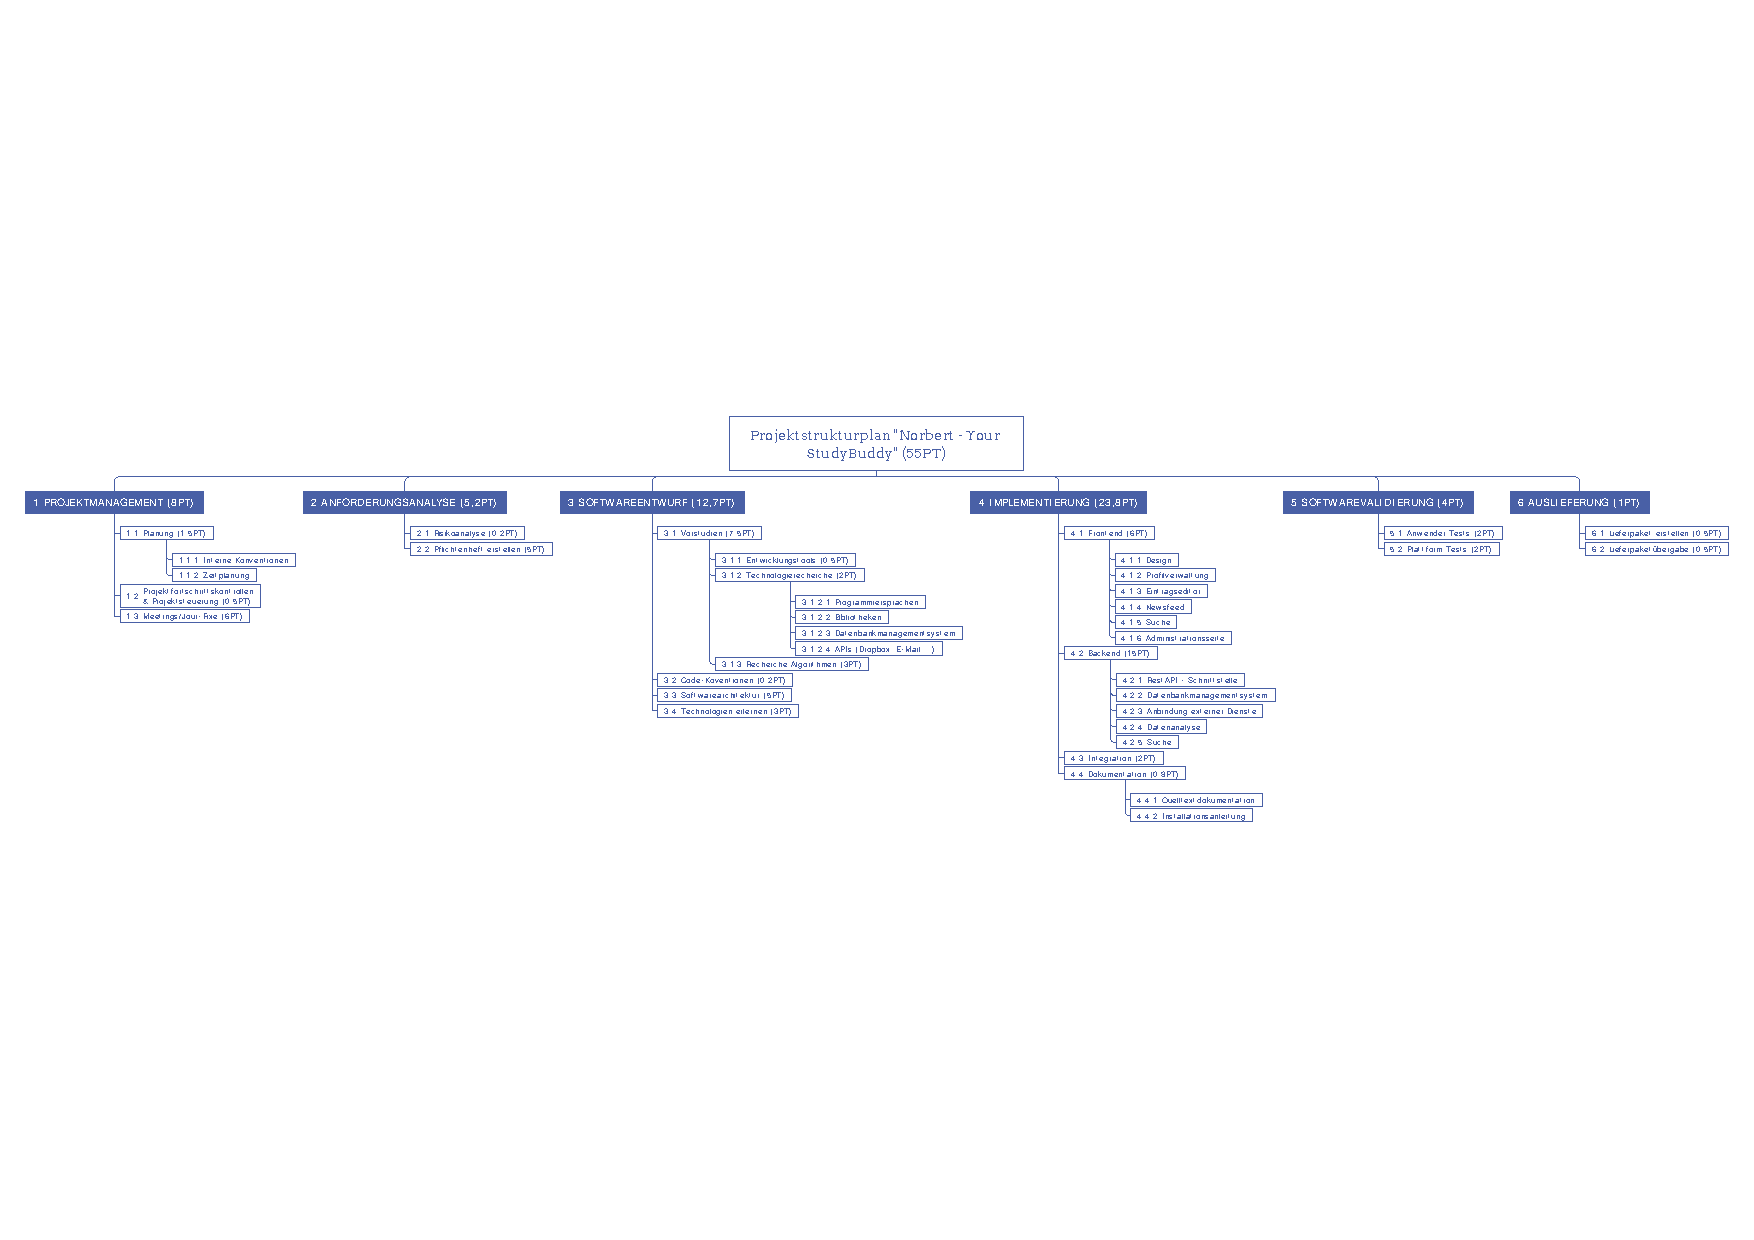
\includegraphics[scale=0.85]{images/plan.pdf}
\end{figure}
\end{landscape}

\begin{landscape}
\chapter{Risikoanalyse}
	Die Spalte \enquote{Eintrittswahrscheinlichkeit} beschreibt, wie hoch die Eintrittswahrscheinlichkeit des Risikos eingeschätzt wurde, wenn keine aktiven präventiven Maßnahmen durchgeführt werden.
	Die Wichtigkeit eines Risikos ergibt sich aus dem Produkt der Eintrittswahrscheinlichkeit mit der Auswirkung beim Risikoeintritt.
	\begin{longtable}{|p{1.5cm}|p{4.5cm}|p{0.4cm}|p{0.4cm}|p{0.8cm}|p{4.5cm}|p{4.5cm}|}

		\hline
		\textbf{ID}
			& \textbf{Risiko} 
				& \begin{turn}{90}\textbf{Eintrittswahrscheinlichkeit in \%}\end{turn}
					& \begin{turn}{90}\textbf{Auswirkung bei Eintritt}\end{turn}
						& \begin{turn}{90}\textbf{Wichtigkeit}\end{turn} 
							& \textbf{Prävention} 
								& \textbf{Lösung} 
		\\ \hline

		RSK-10 	& Ein Teammitglied erkrankt
				& 20 	& 30 	& 6 	& - 	& Die Aufgaben werden so umverteilt, dass die kranke Person von zu Hause arbeiten kann. 

		\\ \hline

		RSK-20 	& Ein Teammitglied muss aus dem Projekt aussteigen. (Zum Beispiel wegen Exmatrikulation)
				& 2.5 	& 60 	& 1.5 	& Sicherstellen, dass keine Wissens- oder Fähigkeitsmonopole entstehen, um die Aufgaben beim Risikoeintritt umverteilen zu können.
								& Die Aufgaben des ausgestiegenen Teammitglieds unter den anderen Teammitgliedern aufteilen.

		\\ \hline

		RSK-30 	& Neue Teammitglieder kommen hinzu
				& 2.5 	& 10 	& 0.25 	& Viel dokumentieren, damit die neue Person schnell eingelernt werden kann.
								& Die neue Person in das Projekt (Projektstruktur und technisches) einlernen und ihr Aufgaben zuweisen, die gut zu ihren Fähigkeiten passen.

		\\ \hline

		RSK-40 	& Anforderungsänderungen - der Kunde stellt ein Changerequest.
				& 20	& 60 	& 12	& Software modular aufbauen, damit sie änderbar bleibt und Puffer für nicht geplante Änderungen einplanen.
								& Das Changerequest wird auf Machbarkeit analysiert. Nach Rücksprache mit dem Kunden wird der Preis erhöht und eventuell der Abgabetermin nach hinten verschoben. Das Changerequest wird umgesetzt. Sollte sich die Änderung jedoch als nicht umsetzbar erweisen und der Kunde das Changerequest nicht zurücknehmen kann oder will, so ist das Projekt gescheitert. Dieser Fall wird gleich behandelt wie das Risiko \enquote{Kunde storniert den Auftrag}.

		\\ \hline

		RSK-50 	& Der Kunde storniert den Auftrag 
				& 0.1 	& 100 	& 0.1 	& Im Projektauftrag wird eine Stornogebühr vereinbart 
								& Der Kunde muss die Stornogebühr bezahlen. Tut er dies nicht, werden rechtliche Schritte eingeleitet.

		\\ \hline
		
		RSK-60 	& Der Kunde ist insolvent und kann nicht zahlen
				& 0.1 	& 100 	& 0.1 	& - 	& Projektende. Sollte das Projekt kurz vor der Vollendung stehen, wird es vollendet und von uns selber vermarktet.

		\\ \hline 

		RSK-70 	& Unsere Entwicklungsgeräte, unsere Testgeräte oder die vom Kunde bereitgestellten Testgeräte gehen kaputt oder werden aus anderen Gründen unbrauchbar.
				& 1 	& 5 	& 0.05 	& Wenn möglich einen Ersatz vorhalten.
								& Auf das Ersatzsystem umsteigen.

		\\ \hline

		RSK-80 	& Daten oder der Quellcode gehen verloren.
				& 0.1 	& 90 	& 0.09 	& Verwendung von Git. So gibt es auf dem Computer jedes Projektmitglieds sowie auf dem Server von Gitlab immer eine volle Kopie des Quellcodes und der Daten und den jeweiligen Dateihistorien.
								& Wo es geht: Datenrettung. Sonst: Neuerstellung der Daten.

		\\ \hline 

		

		RSK-90	& Der Machine-Learning-Algorithmus ist fehlerhaft bzw. funktioniert nicht einwandfrei.
				& 25 	& 40 &	10 	& -
								& Der Algorithmus wird durch Regeln ersetzt.

		\\ \hline

		RSK-100	& Javascript, Node.js, React.js, Bootstrap, Less oder eine andere verwendete Technologie ist zu komplex.
				& 15 	& 50 	& 7.5 	& Präventive Schulungen durchführen und bei der Auswahl von Technologien auf die Komplexität achten. 
								& Die Technologie wechseln oder, wenn das nicht mehr möglich ist, Hilfe von außen holen.

		\\ \hline

		RSK-110	& Schlechter Code oder eine schlechte Architektur verursacht Probleme
				& 15 	& 50 	& 7.5 	& Code-Reviews werden durchgeführt.
								& Refactoring

		\\ \hline
		
		RSK-120	& Es existieren zu wenig Anwender der Software.
				& 20 	& 70 	& 14 	& Marketing betreiben, um Nutzer zu gewinnen.
								& Am Anfang eigenständig Daten in die Software pflegen.

		\\ \hline

	\end{longtable}

	Die fünf Risiken mit der höchsten Wichtigkeit sind RSK-40, RSK-90, RSK-100, RSK-110 und RSK-120. Dementsprechend ist es besonders wichtig für uns, bei der Planung einen Puffer mit einzuplanen und modular zu entwickeln. Außerdem sollten wir plattformunabhängig entwickeln sowie Schulungen und Code-Reviews durchführen. 
	
\end{landscape}
